\documentclass[12pt]{article}

\usepackage{graphicx}
\usepackage{amsmath}
\usepackage{amssymb}
\usepackage{natbib}
\usepackage{amsfonts}
\usepackage{multicol}
\usepackage{float}
\usepackage{oldgerm}
\usepackage{bm}
\usepackage{mathtools}
\usepackage{wrapfig}
\usepackage{fancyhdr}
\usepackage[export]{adjustbox}
\usepackage{xcolor}
\usepackage[shortlabels]{enumitem}

\pagestyle{empty}

\setlength{\headsep}{0.5cm}
\setlength{\oddsidemargin}{-0.5cm}
\setlength{\textwidth}{16.5cm}
\setlength{\textheight}{24cm}
\voffset = -2cm


\pagestyle{fancy}
\fancyhf{}
\rfoot{
\includegraphics[width=1.0in]{cnm.png}}
\lfoot{Homework 2}
\setlength\parindent{0pt}
\begin{document}

\begin{center}
\hfil
{\large\bf {ENGR 2910-101: Circuit Analysis}}
\hfill Instructor: Brian Rashap\\
Midterm 1  \hfill Due: 02/15/23\\
\hrulefill\\
\end{center}

{\bf Question 1} [10] %2.14



\begin{figure}[h!]
\centering 
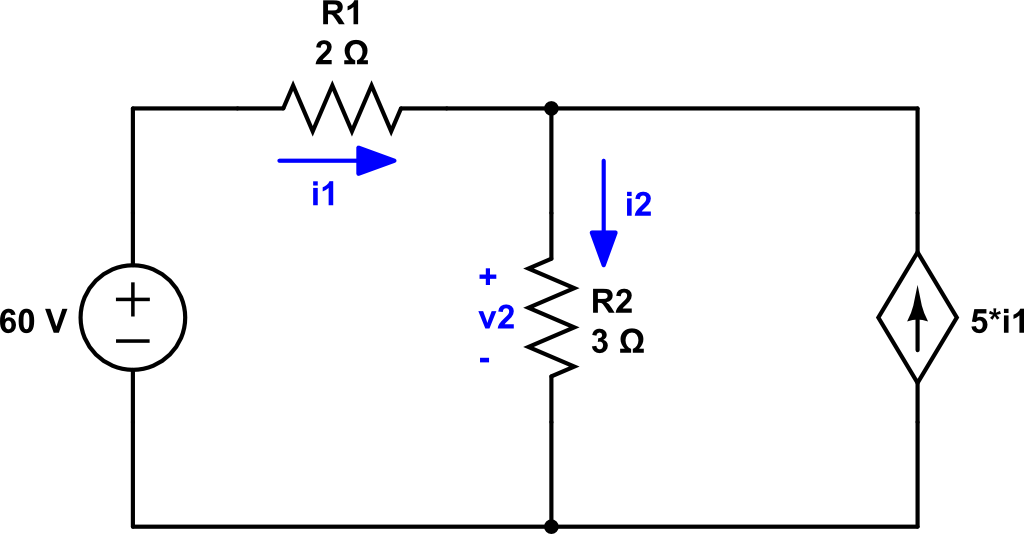
\includegraphics[clip,width=0.49\textwidth]{mid1_1.png}
\end{figure}

{\bf Question 2} [10] %2.18

\begin{figure}[h!]
  \centering 
 \vspace{-0.1in}
 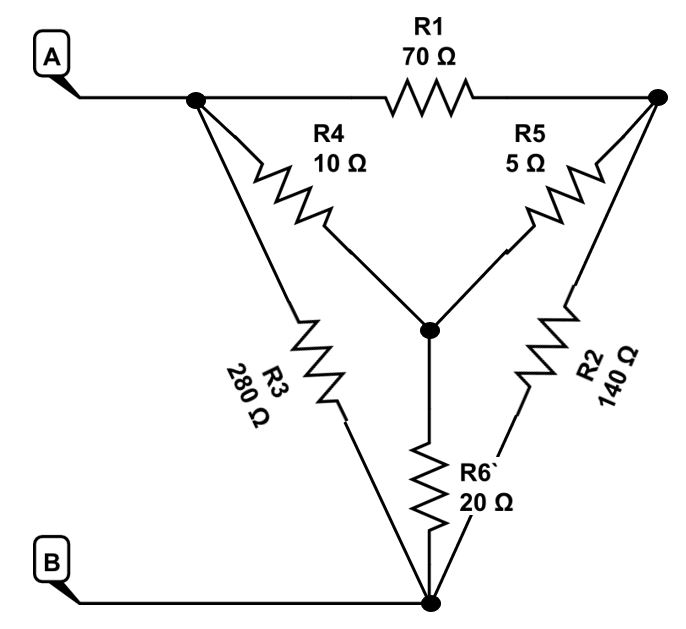
\includegraphics[clip,width=0.7\textwidth]{mid1_2.jpg}
\vspace{-0.1in}
\end{figure}


\newpage
{\bf Question 3} [10] %P2-22

\begin{figure}[h!]
     \centering
\vspace{-0.1in}
       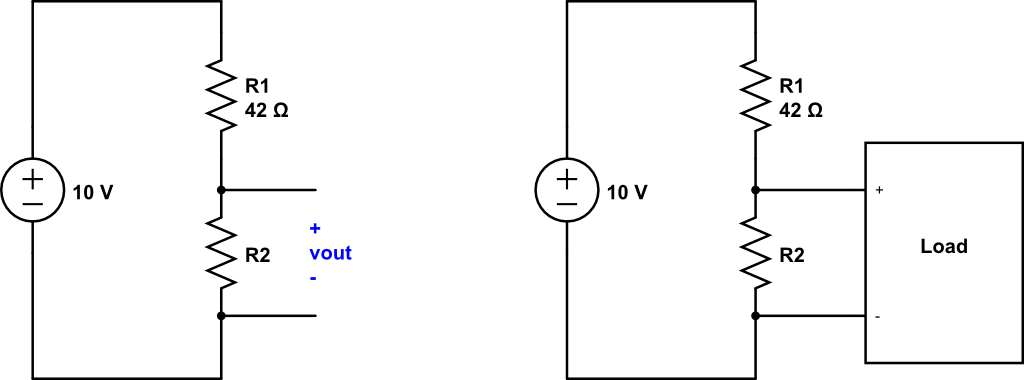
\includegraphics[clip,width=0.6\textwidth]{mid1_3.png}
\vspace{-0.15in}
\end{figure}


{\bf Question 4} [10] %P2-27

\begin{figure}[!h]
  \centering 
  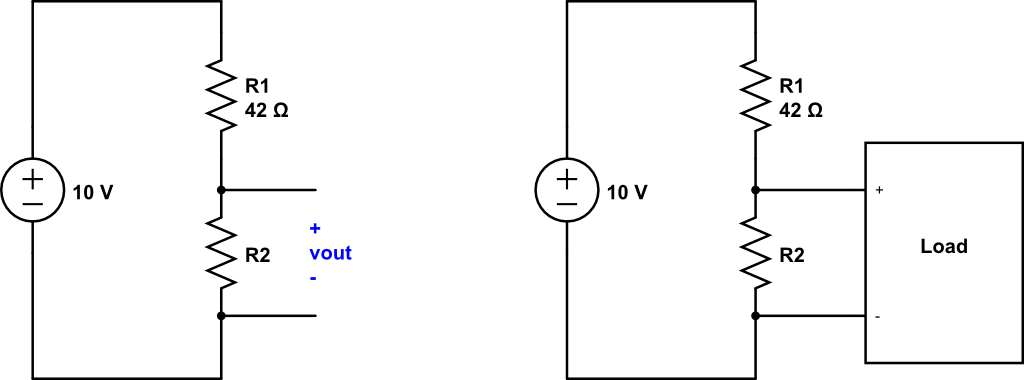
\includegraphics[clip,width=0.6\textwidth]{mid1_3.png}
\end{figure}

{\bf Question 5} [10] %P2-34

\begin{figure}[h!]
\centering 
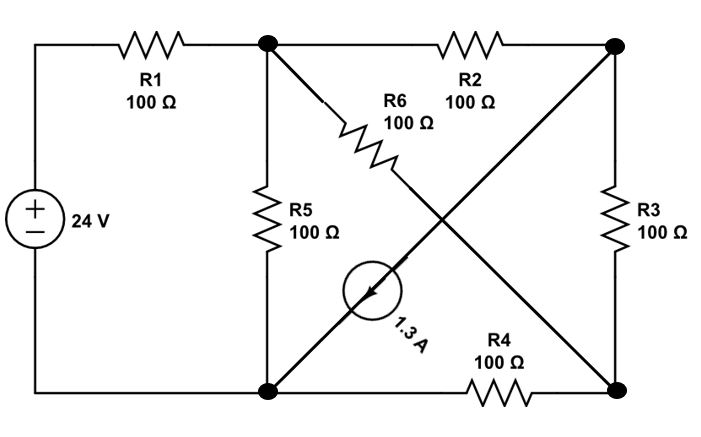
\includegraphics[clip,width=0.6\textwidth]{mid1_5.jpg}
\end{figure}


\end{document}
